\documentclass[12pt,a4paper]{report}
\usepackage[utf8]{inputenc}
\usepackage{textcomp}
\usepackage{amsmath}
\usepackage{amsfonts}
\usepackage{amssymb}
\usepackage{color}
\usepackage{graphicx}

\usepackage{lscape}
\usepackage{rotating}

\begin{document}

\begin{titlepage}

\begin{center}

\textsc{\LARGE Photo Voltaic Cells}\\[1.5cm]

\textsc{\Large PRO4 Project}\\[0.5cm]

\textsc{\Large AU-Herning}\\[0.5cm]


% Author and supervisor
\begin{minipage}{0.4\textwidth}
\begin{flushleft} \large
\emph{Author:}\\
Jacob \textsc{Kristensen}\\
Morten \textsc{B. Koch}\\
Anders \textsc{Bech}\\
Henrik \textsc{H. Christensen}
\end{flushleft}
\end{minipage}
\begin{minipage}{0.4\textwidth}
\begin{flushright} \large
\emph{Supervisors:} \\
Morten \textsc{O. Jensen}
Klaus \textsc{Kolle}
\end{flushright}
\end{minipage}


\vfill

\begin{flushleft}
Summary SHORT
\end{flushleft}

% Bottom of the page
{\large \today}

\end{center}

\end{titlepage}
% \chapter{Executive Summary (Jacob)}
This is a report on the process of analyzing and implementing a Solar Panel system, in close dialogue with the costumer, to get his exact needs for the system-to-be. The customer wants this product as a showcase for high-school visitors, so they can see how to produce green energy.
This report will discuss power line communication, LPC2478 programming and many other exciting topics, in the process of producing this solar panel system, which is only a small part of a bigger, more complex system. Other Teams creates different system parts (modules), which at the end have to work together and interact with each other.
\chapter{Preface (Jacob)}
This report is aimed at lectors and sensors at the Electronic Design Engineering study program at AU- Herning, to share the process of creating the Solar Panel system.
The report was prepared at 3rd and 4th semester of the EDE study, from 08-11 to 05-12. Thank you to classmates and cooperative teams at E10 class for sharing knowledge and experiences when problems occurred, and also for being structured and conscientious when developing the common parts of the project.
The lectors at the AU – Herning has been helpful and willing to help and sharing their knowledge, it is their job to do so, but a big thanks to them for doing a great job teaching has to be given!
\chapter{Version History}

\textbf{0.1}\\
All steps in the launch phase were followed in order to gain knowledge regarding the system that is going to be built.

\begin{itemize}
\item Launch Phase
\subitem The first approach of the report is made.
\end{itemize}

\textbf{0.2}\\

Meeting with the teachers was made, where the discussed topics were: changes and modifications.
\begin{itemize}
\item History added.
\item Summary added
\item Preface added
\item Introduction added
\item Blocks/events updated throughout the entire report.
\end{itemize}

\textbf{0.3}\\

Even more discussion with the teachers gave more additions to the report.
\begin{itemize}
\item Words like “we” and “our” were translated into science language. (3rd person passive)
\item Block Event table, blocks/events switched
\item State Machine Diagram Updated
\item Common Requirement document made.
\item Requirements updated.
\item Design Criteria, safety added.
\item Technical platform updated. Emergency added!
\item Product Acceptance added
\end{itemize}

\textbf{0.4}\\
And a final walkthrough of the Launch Phase report.
\begin{itemize}
\item Grammar and Language revised
\item User needs/requirements updated and corrected
\item Updated Blocks/events
\item Block Diagram Added
\item State machine diagrams added (for all blocks)
\item Update the system interface analysis
\item Updated function analysis
\item Improved requirement analysis
\end{itemize}

\textbf{0.5 (15/12 2011)}\\

Collect pre project, launch phase and realization phase in a single document, updating the intro to the report, to fit all phases.
\begin{itemize}
\item Phases collected in a single document.
\item Structure and order fixed.
\item Introduction updated.
\item Executive Summary Updated.
\item Preface Updated.
\item Problem Statement Updated
\item Introduction to the different phases added.
\end{itemize}

\chapter{Introduction}

\begin{itemize}
\item was the project initiated?
\item ideas, interests and thoughts are behind your choice of subject?
\item others worked on the problem and what did they do?
\item introduction may include artifacts from the PreProject, e.g. Rich Picture. It may fill two pages and cover the problem widely
\item may be a good idea to write this part at the end of a project period
\item Remember to include a list of abbreviations, e.g. in a table under  ”Introduction” or alternatively under ”Appendices”
\item describe how references can be found in the report (i.e. in square brackets).
\end{itemize}

\tableofcontents ???

\chapter{Results}
The artifacts from the EUDP phases are listed in the report under “Results”\\

In EPRO3, this may be the artifacts from PreProject and Launch, and the artifacts from Realization and PostProject in EPRO4\\

Since supervisor or examiner may not be familiar with these artifacts, it is important to include a brief description of what the terms cover\\

Writing reports with EUDP, ver. 0.5 Page 16\\

PreProject is about finding out what needs to be done. The PreProject artifacts are therefore Rich Picture, Storytelling, an overall Use Case Diagram, Stakeholder Analysis, System Definition and PreContracting\\

Launch is about finding out how. The Launch artifacts may be Exact Requirements, Technical Platform, Contracting, an overall Block Diagram as well as an overall Use Case Diagram\\

Realization is about realizing the requirements for Launch. Thus, the artifacts from the Realization phase are the Deployment artifacts from each time box. However, it is important that each artifact is written cohesively in the time boxes to provide a more continuous process in addition to keeping better track of the students’ work\\

The PostProject must include all artifacts\\

The remaining artifacts from PreProject, Launch and Realization must be included in “Appendices”.\\

\section{PreProject}
The pre project is mainly to find out what needs to be done. This is a phase where the customer needs and wishes has to be analyzed and explained in both stories and pictures, in order to compare the customers thoughts with ours, so a common understanding of the project is found.
\subsection{Rich Picture}
This is made to get a common understanding of the system-to-be between and the developers. A rich picture should tell us something about the environment the system-to-be should operate in. The picture must not contain details, only symbols of the different parts the system should contain.\\

The rich picture should not be technical. This will make sure, that even the least technical customers are able to understand, what the drawing is all about. Our job is to describe how we imagine the system, so the customer can see his own thoughts in the picture. We tried to draw a picture of the system, after we have had our first meeting with the customer:\\

First off there are solar cells, which we have to control so it turns towards the sun to get the maximal effect out of it. Secondly there is a storage device, here depicted as a battery, which we have to supply with the solar cells. Finally there is a computer from which we should be able to read out relevant data describing the efficiency of the solar cells.\\

\subsection{Story Telling}
Here we will tell a short story that shows how the system will be to use, and how the environment around the system is.\\

John is not an expert on electricity, but he likes to save money! He wants to install a solar power system that can give him solar power, which he can use in his household. He often has visitors, both adults and children, so the system should be safe, so the curious souls don’t touch the dangerous parts of the system. The control interface of the system also has to be secured, so a child or an animal does not accidentally turn it off.\\

The energy the system produces, also have to be stored in a smart way, so that he will have the energy when he is in need of energy, and not only can use energy when the sun shines.\\

John got his system, and he can proudly show the graphs on his computer, to show family and friends how nice the system is working, and how much money he saves. Also when his friends, who bring their kids stops by, he can talk with the parents, while the kids plays around, without being afraid of the kids destroying the brand new system.\\

When heavy rain will fall, he doesn’t have to give one single thought to the system, because it is secured against the changing weather. And of course he doesn’t have to vacuum clean while the sun is shining; he can do it whenever he wants to, because of the systems function to store energy until it is needed.\\

The system runs without the user’s input. He can check if a green light is on, then it’s all as it should be, and the system is running. If he wants to turn the system off, he can do so. When he turns the system back on, it can be done by a press of a button. The system will handle the rest.\\

To access the information of how much money he saves, he can turn on his computer, and open a window. This will show him a customizable graph. He can choose from a list of data he wants to see, ex. The money saving, how many kWh the system produces or how long until the system is paid off.\\


\subsection{Story cards}

\begin{tabular}{|l|p{12cm}|}
\hline Story Card & test / test \\ 
\hline Name: & Test Card \\ 
\hline Date: & 08/09-2011 \\ 
\hline Project: & PRO4 - Photo Voltaic Cells \\ 
\hline Initials: & JK, MBK, HHC \\ 
\hline Story Description: & Just a few lines to tell what the functuions are used for \\ 
\hline Comments: & Space for comments to the story \\ 
\hline 
\end{tabular} \\
\\
\begin{tabular}{|l|p{12cm}|}
\hline Story Card & test / test \\ 
\hline Name: & Solar panel control \\ 
\hline Date: & 08/09-2011 \\ 
\hline Project: & PRO4 - Photo Voltaic Cells \\ 
\hline Initials: & JK, MBK, HHC \\ 
\hline Story Description: & The sun is moving in a curve across the sky, but not in the same curve every day. The system is able to track the curve of the sun, and points the solar cells towards it, to get a maximal power input. \\ 
\hline Comments: & Space for comments to the story \\ 
\hline 
\end{tabular} \\
\\
\begin{tabular}{|l|p{12cm}|}
\hline Story Card & test / test \\ 
\hline Name: & Voltage conversion \\ 
\hline Date: & 08/09-2011 \\ 
\hline Project: & PRO4 - Photo Voltaic Cells \\ 
\hline Initials: & JK, MBK, HHC \\ 
\hline Story Description: & The battery/storage device needs a constant voltage input, e.g. 50 V, but the output from the solar cells can vary, but our system is able to convert the varying output from the cells, to a constant output to the storage device. \\ 
\hline Comments: & Space for comments to the story \\ 
\hline 
\end{tabular} \\
\begin{tabular}{|l|p{12cm}|}
\hline Story Card & test / test \\ 
\hline Name: & Data logging \\ 
\hline Date: & 08/09-2011 \\ 
\hline Project: & PRO4 - Photo Voltaic Cells \\ 
\hline Initials: & JK, MBK, HHC \\ 
\hline Story Description: & The sun is shining, but how much energy does the system deliver? One can keep track of the efficiency and money savings, by graphs and statistics in a website/program, created from data retrieved by the system. \\ 
\hline Comments: & Space for comments to the story \\ 
\hline 
\end{tabular} \\


\subsection{Preliminary use cases}
This is made so the user can see how the server will respond to his every action.


\begin{tabular}{|l|l|}
\hline \textbf{User} & \textbf{Server}\\
\hline Establish connection to server & Connection Established\\
\hline Request log on to server & Acknowledge logon\\
\hline Request to see graph & Fetching data in graph (Last shown criteria)\\
\hline Show graph for last week & Fetching data for a week in a graph\\
\hline Request log off & Logging off, disconnecting\\
\hline
\end{tabular} 
\\
\begin{tabular}{|l|l|}
\hline \textbf{User} & \textbf{System}\\
\hline Turn on the vacuum cleaner & Discharging battery for stored solar power\\
\hline Turn on the dryer & Not enough solar power, turns on the grid power\\
\hline Dryer and cleaner turned off & Switching back to solar power turns off the grid power.\\
\hline
\end{tabular} 

\subsection{Stakeholder Analysis}
This table is used to clarify who we have to satisfy when we create the solar system. Some have the decision power to tell us what the system should be able to do, while others are the sponsor of our system.
Stakeholder analysis	Has decision power	Has no decision power
Directly involved stakeholder - Involve
Klaus, Morten (Teachers)
Jan (Final customer) - Inform
Team 4
Not directly involved stakeholder - Make happy
Per (Financial funding) As little as possible
Jens (Sales representative)

Klaus and Morten are our teachers, the main leaders of this project. They are responsible for our teaching, and that we do relevant things for our study. We have to do what they say, and they have to know what we do.
Jan is our final customer, and we have to deliver what he wants. We should be in contact with him often, telling him about our discoveries, decisions and progress of the project, so he can tell if we are making the right thing.
Per is the one who sponsor our project, so we have to make him happy, and make the best of what he offers.
Team 4 is us, who creates the project. We have to inform each other about the different parts of the project we do. If one of us creates a part, the other members have to know it, so they don’t do the same, and so their parts fit.
Jens is our sales representative, who buys the parts we need for the project. We just have to inform him what we have to do and what we need.

\subsection{System Definition}
The system definition should be able to tell exactly how the system should work, what different parts the system contain and how they should work together, but still without all the technical descriptions.
We have our solar panels, where the energy from the sun, is transformed into electricity. The voltage will be converted to fit with the needs from the power hub, from where the electrical energy is used. If the sun does not shine, all the electrical equipment will get power from the power grid, and when the solar panels are producing more energy than is used, it is stored.
All the energy running through the system will be measured and stored on a server, where a computer can sketch the data in graphs. This will show the user how much energy and money he has saved on green energy.
The system will measure the direction of the sun, and then the solar panels will be pointed in that direction so the outcome will be as high as possible.
\subsubsection{Weather conditions}
Some parts of the system have to be outside, so it should resist the different weather conditions, without taking damage.
\subsubsection{Curious visitors}
Some of the visitors of the owner may be curious. Children, and some adults, may mess with the system. The weak parts of the system should be protected from animals and children touching it.
\subsubsection{Convert voltage to desired output}
Another part of the development department has to construct the storage device for the power, so the output voltage of our system has to fit their part of the system.
\subsubsection{Plot important data}
We have to collect useful data from our system and store then, so we can plot it in a graph. This makes the customer able to see the outcome and savings in a way he can understand.
\subsubsection{Right Position}
The solar cells have to point in the right direction, to make the maximal power. The system has to keep track of the suns position, and rotate the panels to the right position.
\section{Launch Phase}
Now an understanding of what we have to create in the project has been made, so now it is time to find out how it have to be made. The Launch Phase will provide a detailed analysis of the project. The exact requirements have to be found, in order to know exactly what the system has to fulfill to satisfy the user’s needs.
\subsection{General Analysis (Jacob)}
In this Phase the requirements for what is needed in the system is found. There will be determined, how it shall interact with the environment and how the user should interact with the system. The system-to-be should be seen as a black box, the user can’t see how it works in details, and the user can only see which different parts it has to contain for the system to work probably. This is the initial analysis.
The next step is to open the black box, look inside and use the requirements found in the step before, to determine which requirements the system-to-be has to meet. If those requirements are met, the system will fulfill the user needs
The system Overview diagram is shown below:

\subsubsection{Block Analysis (Jacob)}
\textbf{Block Candidates}\\

First the user sees the system as a black box, or a lot of black boxes. The system is divided into blocks for easier explaining. These blocks represent different parts of the system, which have different functions. A banana for example exists of two parts, the outside shell (block) which protects the inside (function). The inside (another block) is to be eaten and to get rid of the hunger (function).\\

The first thing declared is what parts of the environment is required for the system to work when it is created. A model of the important parts of the environment is created. An abstraction of the environment is created, in order to create an easier overview of the system-to-be. If for example the system has to control the temperature in a pool, a sensor that measures the temperature of the water makes sense for the system.\\

“Definition: Block - A Block defines an object's interface and implementation. It specifies the object's internal representation and defines the operations the object can perform...”\\

Below is the brainstorm of block candidates for our system.\\

\begin{itemize}
\item Battery(Part of another groups system)
\item SolarPanel
\item Computer(To connect to the webpage, not included in our system)
\item PowerGrid(We can’t send electricity to the powergrid, too dangerous)
\item DataServer(A common part for all teams. Outside our system)
\item LPC2478 (A part of other blocks)
\item TheSun (Not a part of our system, but the environment)
\item SunTracker
\item Regulator
\item MotorDriver
\item Communicator
\item EnergyHub (Another teams system)
\item Logger
\end{itemize}

TheSolarPanel is a Block, that is necessary for the system to work. The panels function is to absorb energy from the sun, and turn it into electricity.\\

The second Block added is the SunTracker. To get the maximal energy from our panel, it has to point directly at the sun. This tracker has to measure where the sun is positioned.\\

MotorDriver makes the panel point in the right direction, by turning the panel, in that direction the SunTracker measures is the right.\\

The Regulator regulates the power retrieved from the panel. The power is afterwards send directly to the energy hub, that’s why it is important, that the voltage/current is regulated.\\

The Communicator is the only block which can communicate with the energy hub. All communication is sent through the communicator block.
The Logger reads information about how much the panel is producing, and collects the information in a package. This package is then sent to the hub, through the communicator.\\


\textbf{Event Candidates}
Event candidates which are the events occurring at different times, which change some kind of variable for the classes, if for example the SunTracker measures a change of the suns position, it has to interact with the Motor classes, to adjust the SolarPanel.\\

“Definition: Event - An instantaneous occurrence that will influence on one or more objects.”\\

\textit{SunTracker}
\begin{itemize}
\item PanelInPosition
\item PanelNotInPosition
\item TurnOn (May not be necessary)
\item TurnOff (May not be necessary)
\item ReadPosition
\subitem When a delay has run out, the tracker will read the position to the sun. After the position is read, they are sent to the MotorDriver, which turns the panel into the right position and angle to the sun.
\item ProductionStart (Described here, used in different modules)
\subitem Production is turned on, the system shall run the delay().
\item ProductionStandby (Described here, used in different modules)
\subitem When production is turned off, the block has to use as little power as possible.
\item SystemReady (Described here, used in different modules)
\subitem When the module is powered on, it has to initialize. When initialized, it is ready, and moves to next state.
\item SystemOff (Described here, used in different modules)
\subitem Event occurs if emergency button is pressed, or if module is powered off. This event will cut off power to the module.
\end{itemize}



\textit{Regulator}
\begin{itemize}
\item ProductionStart
\subitem Production has to be turned on, as mentioned before, but the sunlight limit also has to be equal to or above the limit.
\item ProductionStandby
\subitem The module also has to turn off, if the sunlight is below the limit. If this happens, the regulator will not be able to regulate to the desired output. 
\item SystemReady
\item SystemOff
\item InputRegulated
\item InputNotRegulated
\end{itemize}


\textit{MotorDriver}
\begin{itemize}
\item ProductionStart
\item ProductionStandby
\item SystemReady
\item SystemOff
\item PanelPosition
\subitem The MotorDriver has to adjust the angle to the sun, every time a delay runs out. The panel is positioned prior to the read coordinates from the Suntracker.
\end{itemize}


\textit{Communicator}
\begin{itemize}
\item ProductionStart
\item ProductionStandby
\item SystemReady
\item SystemOff
\item PingRecieve
The hub will ping the device, to ensure a connection is established, to avoid serious system failure. The system has to answer the ping, to know the connection is established. 
\item PackageReady
When the system is receiving a ping and a package is not ready for delivery, a signal should tell the hub to continue to ping the next system.
\end{itemize}


\textit{SolarPanel}\\
The solar panel doesn´t have any events, this is always on. The user can’t start/stop the production at this part.



\textit{Logger}
\begin{itemize}
\item ProductionStart
\item ProductionStandby
\item SystemReady
\item SystemOff
\item SampleOutput
The system has to record how much power is sent to the hub, so the user can see a production graph at his webpage. Every time the SampleDelay has run out, the system has to sample the input and output of the system.
\item PackageReady
When a PackageDelay has timed out, all collected data has to be sent to the data server. The system has to tell the hub to bring the package to the data server. The hub acts like a delivery boy.
\end{itemize}

\textbf{Block Event Table}\\
In the Block event table Blocks and events are linked together if they have any connection.

\begin{tabular}{|l|l|l|l|l|l|l|l|l|l|}
\hline Blocks \ Events & SystemReady & ProductionStart & ProductionStandby & SystemOFF & PackageReady & SampleOutput & PingRecieve & PanelPosition & ReadPosition \\ 
\hline SunTracker & X & X & X & X  &  &  &  &  &  X \\ 
\hline Regulator & X & X & X & X  &  &  &  &  &  \\ 
\hline MotorDriver & X  &  &  &  X  &  &  &  &  X  & \\ 
\hline Communicator & X & X & X & X & X  &  &  X  &  &  \\ 
\hline SolarPanel &  &  &  &  &  &  &  &  &  \\ 
\hline Logger & X & X & X & X & X & X  &  &  &  \\ 
\hline PLC Device &  &  &  &  &  &  &  &  &  \\ 
\hline 
\end{tabular} 


\textit{Block Diagram}
The Block diagram shows the relation between the different blocks in the system. 

\begin{figure}[htbp]
\centering
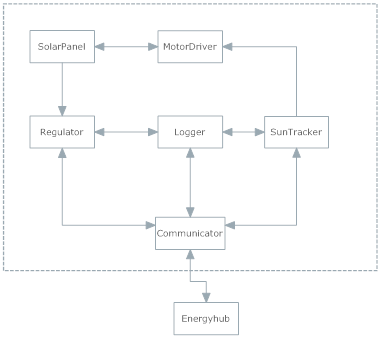
\includegraphics[width=20px]{images/blockdiagram.png}
\caption{}
\label{fig:BlockDiagram}
\end{figure}


\textit{State Machine Diagrams}
It is not only important to know which blocks will interact with eachother, it is also important to know, how every single block is built up. The state machine diagram will shows what is inside the block and what events triggers what functions:

\begin{figure}[htbp]
\centering
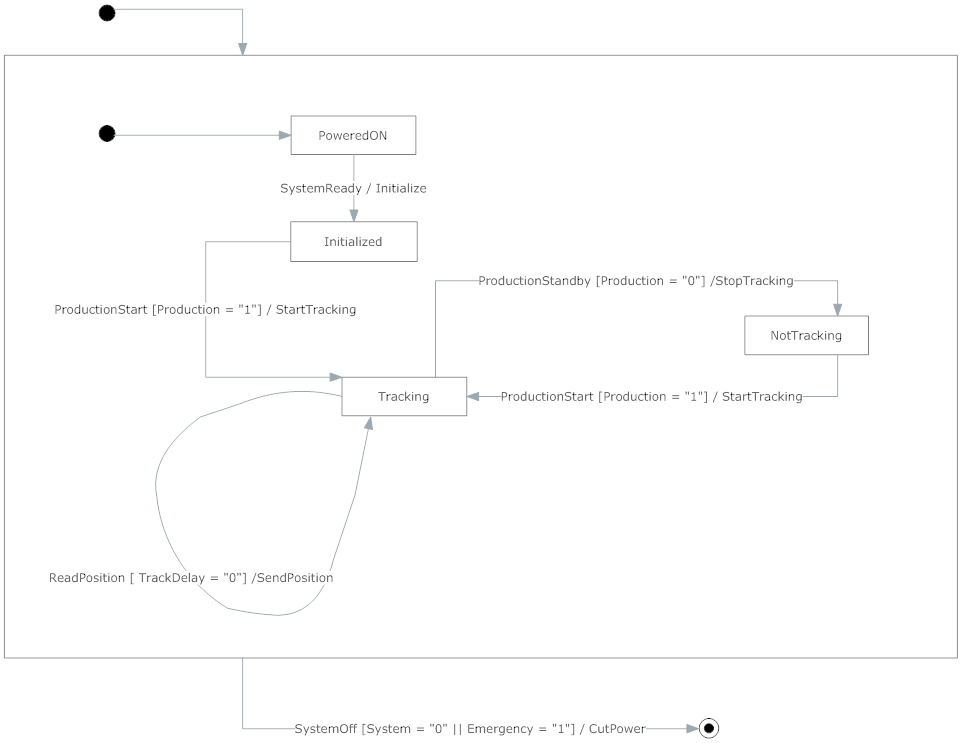
\includegraphics[width=8cm]{images/SunTrackerUML}
\caption{State Machine Diagram of SunTracker}
\label{fig:SunTrackerUML}
\end{figure}



All modules start in the state “PowerON”. When the system is ready it will initialize, it will move on to the state “Initialized”. When the block gets a signal to start production, the system will move on to its “initial” state.
Another common state is the “StandBy” state. The stand by state of the Tracker is the “NotTracking” state. If the system gets a signal to set the production on stand-by, it will move to the state “NotTracking”, where it will wait for a signal to start production again. Those signal about start and stop production are given by the hub, which the power is sent to.
All Blocks also contains a “SystemOFF” event, which will occur if the power is cut, or if the emergency button is pressed.
The initial state of the SunTracker is the “Tracking” state, where a TrackDelay will count down, and measure the position of the sun, and then reset the delay counter. After the position is measure, it will be sent to the MotorDriver.

\begin{figure}[htbp]
\centering
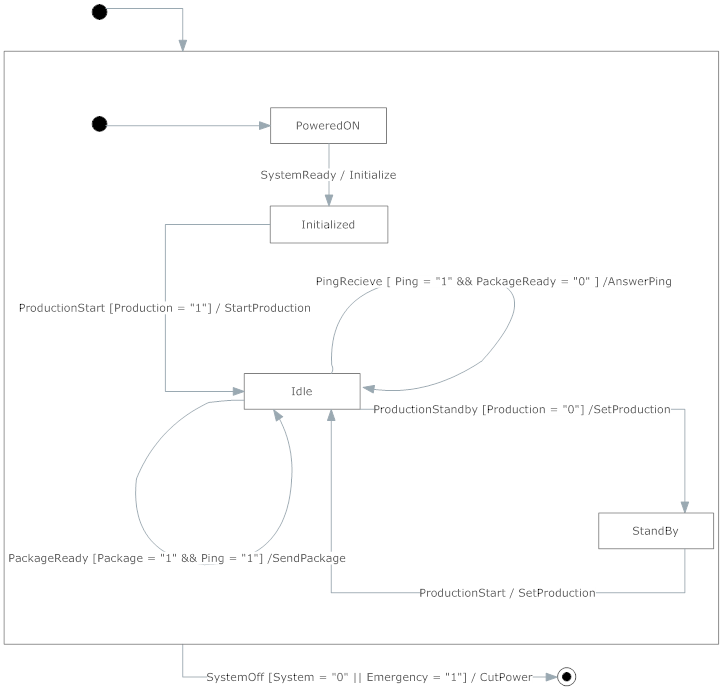
\includegraphics[width=8cm]{images/CommunicatorUML}
\caption{State Machine Diagram of Communicator}
\label{fig:CommunicatorUML}
\end{figure}


When production starts, the Communicator will listen until a ping is received, or a package is ready to be sent to the hub. If a ping is received, and a package is ready, the Solar Module will answer by sending the package to the hub. It a ping is received, and no package is ready for the hub, the module will answer with an empty package, just to inform the hub, that the module is alive, and the connection is not lost.

\begin{figure}[htbp]
\centering
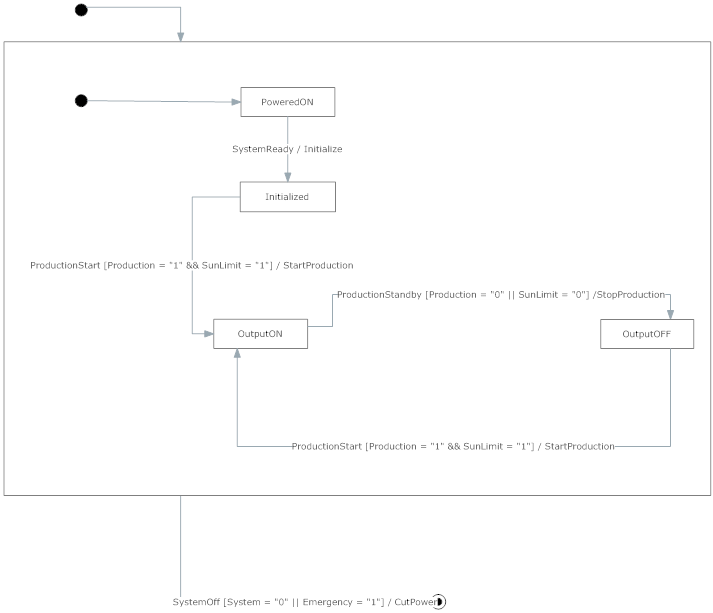
\includegraphics[width=8cm]{images/RegulatorUML}
\caption{State Machine Diagram of Regulator}
\label{fig:RegulatorUML}
\end{figure}


The regulator block can turn its hardware on or off, according to the production status. The regulator is made of pure hardware, and no software will regulate the output to the hub, it will only measure if it is regulated to the right values, and in case it is not, the output is turned off.

\begin{figure}[htbp]
\centering
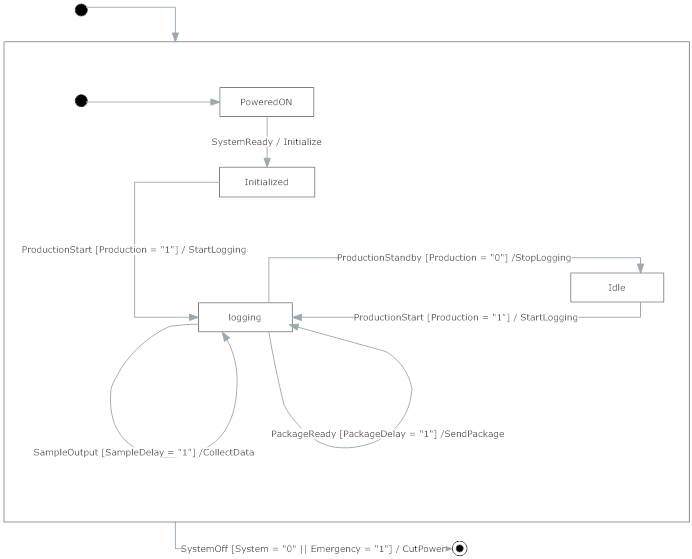
\includegraphics[width=8cm]{images/LoggerUML}
\caption{State Machine Diagram of Logger}
\label{fig:LoggerUML}
\end{figure}


The logger runs two delays. The first delay is the “SampleDelay”. When this delay runs out, the logger will sample the necessary data from the regulator, the solar panel and the sun tracker. Then the delay will reset, and count again. The “PackageReady” delay will prepare a package to the hub every time it runs out. The hub has to receive data to the web-server with a given interval, so the web-interface can be updated. When the delay runs out, the sampled data has to be collected in a file. Then the logger has to inform the communicator about the package waiting to be sent to the hub.

\begin{figure}[htbp]
\centering
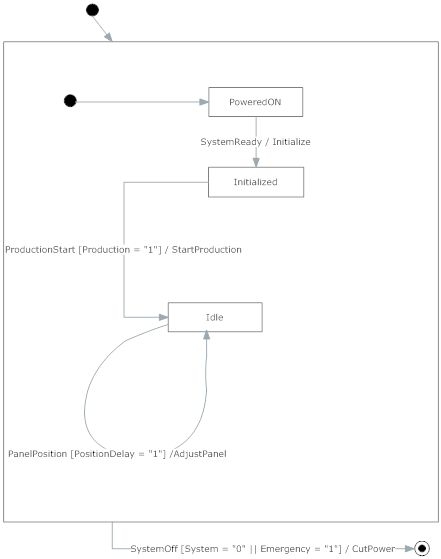
\includegraphics[width=8cm]{images/MotorDriverUML}
\caption{State Machine Diagram of MotorDriver}
\label{fig:MotorDriverUML}
\end{figure}


The position of the sun is logged by the sun tracker, and every time the “PositionDelay” runs out, the motor driver has to position the solar panel according to the position of the sun. By inserting a delay, the panel will be adjusted with a given interval, instead of making the motor driver position the panel every time a new position is received. This interval can either be constant, or vary from sun rise to sun set. The sun “moves faster” in the morning and evening than it does at midday.

\subsubsection{Use Case Analysis (Morten)}
\textbf{Use Case Candidates (Customer Meeting)}
The Use Case Candidates are the different actions the user can change during the use of the system. We had a customer meeting with our customer, to see what he had in mind. He gave the following candidates:

\begin{itemize}
\item Emergency stop system
\item View all data daily
\item View all data weekly
\item Configure solar power production (ON/OFF)
\end{itemize}

\textbf{Actor Candidates}
The Actor Candidates are the people that will use the system now or in the future. The production test engineer makes and tests the system, the customer uses it as a benefiting product and the service technician will be contacted in case of errors.

\begin{itemize}
\item Service Technician 
\item Customer
\item Production test engineer
\end{itemize}

\textbf{Use Cases}
The Use Case will show a simple case where the user interacts with the system in some kind of way. We can see the users actions and how the system responds to said action

\begin{tabular}{|l|l|l|}
\hline Number & Actor & System \\ 
\hline 1 & Select to view data in graph &  \\ 
\hline 2 &  &  (last known configuration) \\ 
\hline 3 &  & Display the graph \\ 
\hline 4 & Select to view data in a monthly periode &  \\ 
\hline 5 &  & Fetches data and updates graph \\ 
\hline 6 &  & Display the updated graph \\ 
\hline 7 & Happy Costumer &  \\ 
\hline 
\end{tabular} \\
\begin{tabular}{|l|l|l|}
\hline Number & Actor & System \\ 
\hline 1 & Press emergency button &  \\ 
\hline 2 &  &  System power off immediately \\ 
\hline
\end{tabular} \\
\begin{tabular}{|l|l|l|}
\hline Number & Actor & System \\ 
\hline 1 & Chooses to stop production &  \\ 
\hline 2 &  &  Modules enters "idle" state \\ 
\hline
\end{tabular} \\
\subsubsection{Interface Analysis (Morten \& Jacob)}
\textbf{User Interface analysis}\\

The User Interface analysis shows a simple prototype of the interface of the system-to-be, here you can see a typical graph with a changeable unit and a changeable period.

\begin{figure}[htbp]
\centering
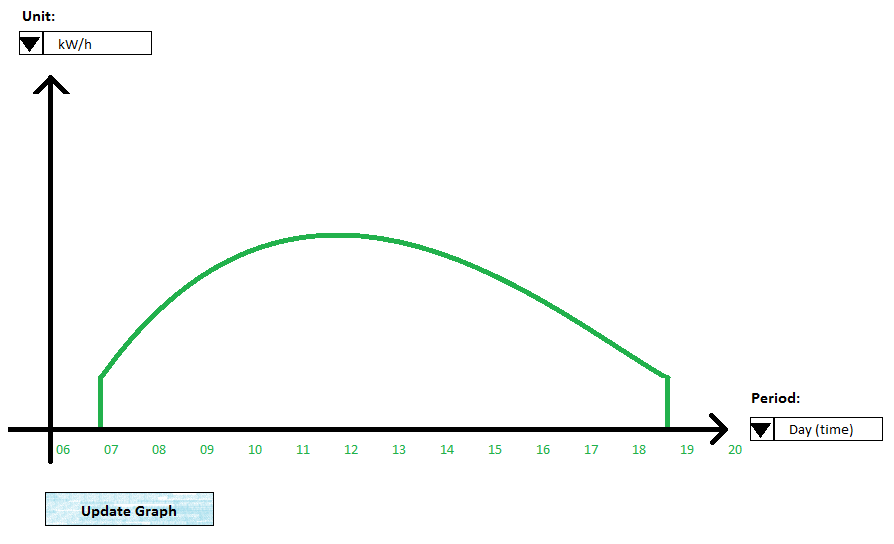
\includegraphics[width=8cm]{images/SampleGraph}
\caption{Sample Graph}
\label{fig:SampleGraph}
\end{figure}


Select the desired x- and y axis, to see the given unit in the desired period.
Then click “update graph”, to update the graph.
Scenario: Let the users choose the values and click update, then change the graph accordingly.
Those data will be able to see at the webpage we will create in corporation with the other teams. A representative from each team will be chosen who should attend to meetings, where the web design was discussed, among other things.
The customer chose to use a webpage as the interface between our system and the user. He also wanted a physical control panel to shut on/off different parts of the project. But he can find the graphs and other data only at the webpage, where he will also be able to turn on/off the parts.
Below you can see the solution for the web design we have developed so far, together with the other teams. We have not represented it for our customer yet, but we have booked a meeting, where he will give us his opinion about the interaction design.
First we have a picture of the first page you will meet. Here you can see the energy hub, and the buttons to enter ex our page with information about the solar panel production. Here you also can turn on/off the different parts if you are logged in.

\begin{figure}[htbp]
\centering
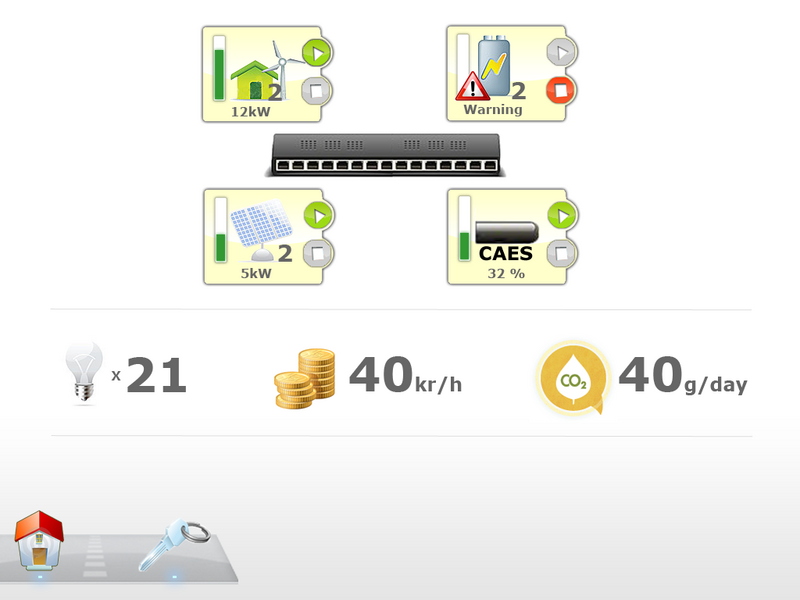
\includegraphics[width=8cm]{images/frontpage}
\caption{Frontpage}
\label{fig:800px-Frontpage_public}
\end{figure}


The next image is a page for an individual part. This picture below shows the page for the energy hub.

\begin{figure}[htbp]
\centering
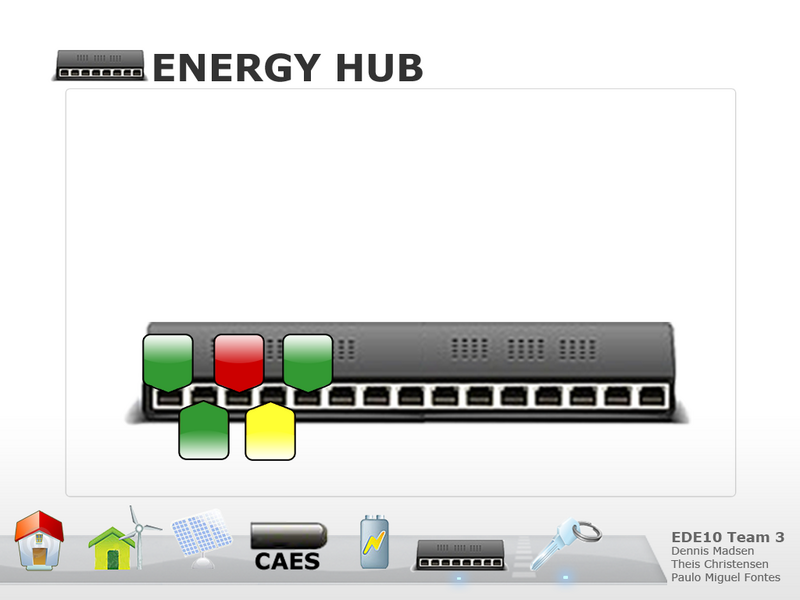
\includegraphics[width=8cm]{images/submodulepage}
\caption{Energy Hub Frontpage}
\label{fig:800px-Submodule_page}
\end{figure}

The user can easily see that you have entered the energy hub page, by looking at the header. The user can enter the other parts directly by choosing them at the bottom dock. Images make it all user friendly, and everybody can see, that they should press the picture of the solar panel to enter the information about the solar panel.\\
\textbf{System Interface analysis}

\begin{itemize}
\item Emergency button
\\If the user discovers smoke or fire inside the system, a big red emergency button should be able to cut off all the power to the system.
\item ebpage
\\This is as described above, where he can see system information and turn on/off different parts.
\item PowerLine communication
\\Powerline communication is used to transfer data between the different systems, example from our solar panels to the energy hub. Powerlines is also used to transfer energy from the solar panel. 
\item Output voltage to hub
\\As mentioned above, the powerline also is the interface to the power transfer. 
\item The hub is constantly pinging our system, if this ping isn’t received,our system will shut down, with a status message saying:”Communication Lost”.
\end{itemize}

\subsubsection{Function Analysis (Jacob)}
\textbf{Function Candidate Analysis}

\begin{itemize}
\item UpdateGraph()
\item CalcTalkTime()
\item Production()
\item System()
\item CalcBulbs()
\item CalcCoffee()
\item Ping()
\item SendPackage()
\item Production()
\item Initialize()
\item Idle()
\item AdjustPanel()
\item ReadPosition()
\item SendPosition()
\item Production()
\item Initialize()
\item SendPackage()
\item Idle()
\item CollectData()
\item Logging()
\item PassPackage()
\item UpdateWeather()
\item Regulate()
\item CalcWatt()
\end{itemize}

\subsubsection{Function Analysis}
\textbf{Communicator}\\
The only way the system can communicate with the hub, is through the communicator. Several functions will be used.
The hub will ping the solar module with a fixed delay. Then the module will know if the communication is lost or not, to ensure important communication can pass. Every time a ping is received from the hub, the solar module has to answer it.
The system also collects data about the production, which will be sent to the server, through the hub. A SendPackage() will be needed, both to send the package, and to receive an acknowledge bit, to know if the package is sent or lost.
\begin{itemize}
\item AnswerPing()
\item StartModules()
\\When the communicator receives a package from the logger, it enters theSendPackage() and sends it to the hub. Here it waits for an acknowledge bit, to be sure the package is received.
\item Initialize()
\item SendPackage()
\item Idle()
\end{itemize}

\textbf{User} \\
% \LEFTarrow \\
% \RIGHTarrow \\
\textbf{System}\\

The user can do several things to interact with the system. At the web-page, he can update graph, and convert the data into more pedagogical numbers, such as “how many light bulbs can the system light up right now?” And also calculate in coffee cups and talk time on a cell phone.
Some common functions for several modules is the production() and the system(). First the user has to power on the system, which activates the initialize(). This will send the system into idle state, and wait for orders to start production().
When the system is initialized, the user can start production(), and the system will move on from the initial state and begin production. Every active module has their own initialize() and idle() function to start up, initialize and start production.\\

\begin{itemize}
\item UpdateGraph()
\item CalcTalkTime()
\item Production
\item System()
\item CalcBulbs()
\item CalcCoffee()
\end{itemize}

\textbf{MotorDriver}
\\The motor driver will wait in idle state for a new position to mirror. When the position is received, the AdjustPanel() will reposition the panel.

\begin{itemize}
\item Initialize()
\item Idle()
\item AdjustPanel()
\end{itemize}

\textbf{SunTracker}
\\Every time a TrackDelay runs out, the system will ReadPosition() of the sun, and send this position to the motor driver. Also a send delay is counting. It has to read data and collect them into a package, which it sends to the hub every time a logger delay runs out.

\begin{itemize}
\item Initialize()
\item Idle()
\item ReadPosition()
\item SendPosition()
\end{itemize}

\textbf{Logger}
\\The logger also reacts on a LogDelay. After this delay, it has to enter Logging() to log the input and output of the regulator, and CollectData() in a package, which is passed on to the communicator.

\begin{itemize}
\item Initialize()
\item Idle()
\item CollectData()
\item PassPackage()
\end{itemize}

\textbf{Regulator}\\
When the user activates the system, the regulator will begin to regulate the power from the solar panel, and send the output to the energy hub. 

\begin{itemize}
\item Initialize()
\item Idle()
\item Regulate()
\end{itemize}


\begin{figure}[htbp]
\centering
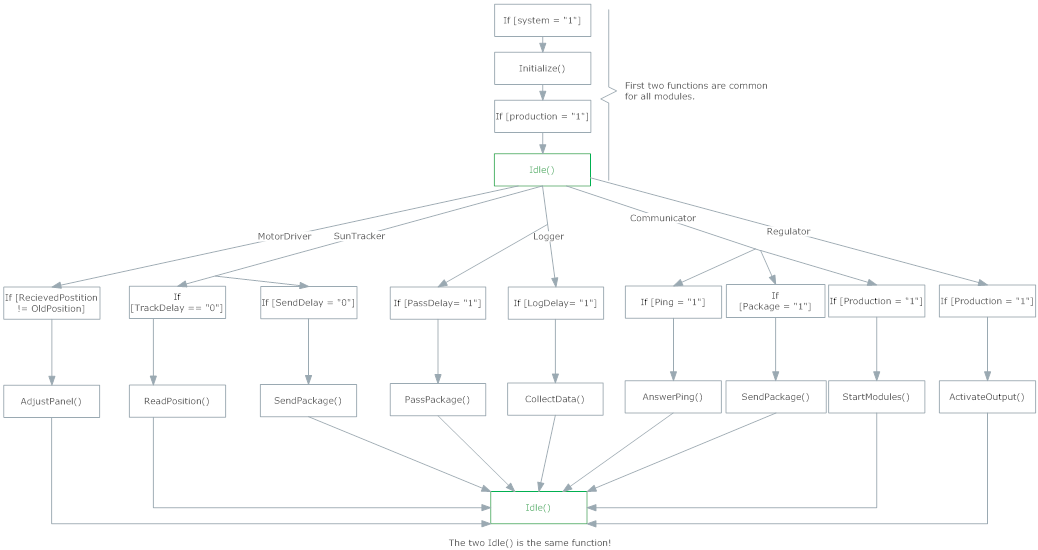
\includegraphics[width=8cm]{images/functiondiagram}
\caption{Function Diagram}
\label{fig:FunctionDiagram}
\end{figure}



\subsubsection{System Dynamics (Henrik)}
\textbf{Communication Diagram}
This diagram illustrates the communication lines within the system and with the user. The dotted lines separate the system into three major communication areas; the web communication out to the user (upper left), the system’s internal data-communication (lower left) and the more hardware related communication (right side).

\begin{figure}[htbp]
\centering
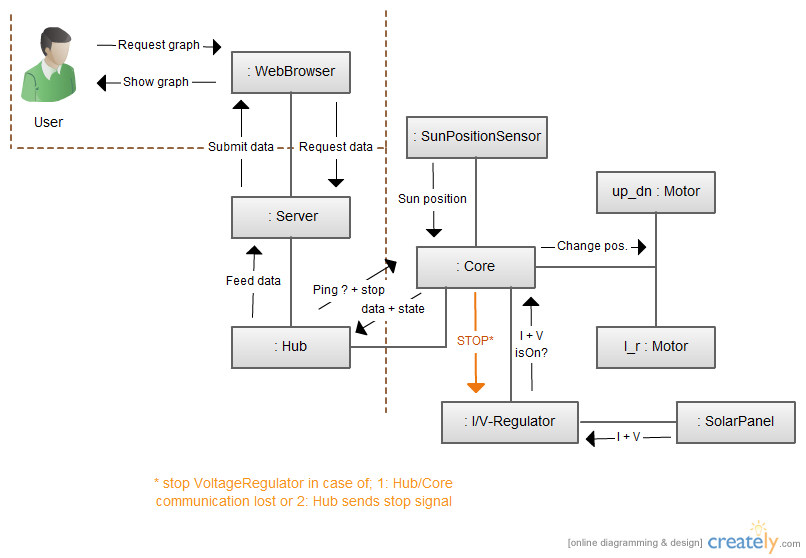
\includegraphics[width=12cm]{images/communicationdiagram}
\caption{CommunicationDiagram}
\label{fig:CommunicationDiagram}
\end{figure}


\textbf{Sequence Diagram}
While the previous diagram shows how the communications run in the system, this diagram is simplified and shows how the communication goes in real-time.

\begin{figure}[htbp]
\centering
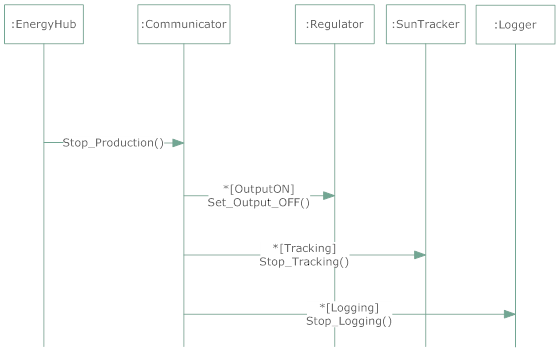
\includegraphics[width=8cm]{images/SequenceDiagram}
\caption{Sequence Diagram}
\label{fig:SequenceDiagram}
\end{figure}


The user may at any time choose to see a graph involving his data in the desired time interval, his input will be accessed via the interface, then sent to the server code which will calculate the data so it will only show the right amount and then it will fetch the desired data and send it to the user in a visual graph. 	

\textbf{Requirement Analysis (Jacob)}
In order to specify the exact requirements you need to locate, analyze and describe the needs of the customer in an iterative process.

\textbf{Customer Requirements / Needs}
Of course the system must be safe to use. When the user turns the system on, it will find the right angle to the sun, by turning around. If there are people around, they must be safe not to be injured by the moving parts. The system has to be placed away from where people stay.\\

A manual turning function is to be implemented too, so users can turn the panel, and see which effect that has on the output. Both the safety mentioned before has to be applied here too, but also a system safety, so the panels can’t turn more than the parts can handle. The system must not burn down or break, because of the manual turning function. It has to stop at maximum turning angle.\\

The spot where the panel is to be placed has to be right, not just for safety sake, but also to get best output possible. It has to be placed somewhere sunny, with no trees or structures covering it up. The panel must get as much sun as possible.\\

Where the sun is shining, the rain is falling. The solar panel, and the other parts of the system that have to be placed outside, have to be resistant to the given weather conditions; resistant to water and able to work in both hot and cold weather.\\

The dangerous parts of the system must be shielded of so no curious visitors can get injured by being around. If they want to control the system, they have to get administrator rights to a web-interface, where all “production start/stop” commands are given. But if they only want to see the data of the system, they can access it on the web-page without administrator rights.\\

If the user desires to turn the panel manually, the physical control panel is to be used. To turn the panel, you will need a key, to unlock the panel. This is for safety reasons. Only people allowed to operate the panel should be able to.\\

If there against any odds should appear smoke, or even fire inside the system, an emergency button must be implemented, to shut down the system instantly, to avoid more damage than necessary.\\

The system can be turned on/off, when the user wants to do so. Our  is not the only user; he will get high-school students as visitors, who also have to work as users. A few days before those visitors come by, the will turn the system on, to get data of the panel’s production. Then the visitors can see how much the system produces on an average day.\\

The customer needs a system which is able to function in 8 years, without major parts has to be replaced. Small components, which are easy replaceable can be replaced if necessary.\\

High-school students are the users, which mean the system must be simple to use and operate. Also the web-interface has to be simple and easy to use and navigate.

\begin{itemize}
\item The system shall be safe to operate.
\item The panel shall be placed, where unauthorized persons can’t access it.
\item The panel shall be placed in a sunny place.
\item The panel shall resist weather conditions.
\item Only the web-interface shall be accessible for all visitors.
\item Visitors can turn the solar panel manually from a physical control panel.
\item Only web-interface and physical control panel shall be operated. 
\item The system will be on for user chosen periods of time.
\item The system will be used for 8 years.
\item The system control shall be easy to use.
\item The system interface shall be simple to navigate.
\item See common requirements .
\item An emergency button shall be implemented.
\end{itemize}

\textbf{Functional Requirements (System shall do)}\\

The system must be easy to use, and should be as automated as possible. All manual system controls is implemented on the energy hub, so the user can start and stop the different modules from the same control interface. Then the hub automatically sends orders to the modules. The modules must accept and follow these orders.\\

All the power our module is producing must be sent through powerline communication to the energy hub. The power must be converted to the right voltage and current. Then the energy hub will send the power to one of the two storage devices.\\

To get as high power output as possible, the solar panel must be in the right angle to the sun. For this we will need some kind of mechanism to reap the suns position, and turn the panel into position.\\

When the user wants to see a graph at the web-page, some data has to be logged. These data is logged by our system. It logs both the output from the solar panel before it is converted and after it is converted. Also the intensity of the sun is logged, to compare with the output. And the same is done for the angle to the sun. Those data is sent to the hub, which passes them to the data server, wherefrom the web-page can read them.\\


\begin{itemize}
\item The system shall track the position of the sun.
\item The system shall sync the direction of the panel with the direction of the sun.
\item The system shall convert solar power into electrical power.
\item The system shall regulate its output.
\item The system shall log the output voltage.
\item The system shall read the sun intensity.
\item The system shall log the sun intensity.
\item The system shall obey orders from the energy hub.
\end{itemize}

\textbf{Non-Functional Requirements / Performance Requirements (system shall be)}
\begin{itemize}
\item See common requirements.
\end{itemize}

See common requirements.

\subsection{General Architecture Design}
\subsubsection{Design Criteria (Morten)}
The following categories are categorized in the matter of its importance: Performance, Usage, Reliability, Easy serviceable, Remote maintenance, Cost effective, while of course all of them are required for the system to be, one or two might have a higher focus value. The system will be as reliable as possible, if at any chance an error occurs we will send maintenance people to change selected HW or SW making it easier for the customer to enjoy the product. The system will be made of mostly electronic yet made in a simple planner so the customer will experience an easy usage of the product.\\


\textbf{Criteria:}\\
\begin{tabular}{|l|c|c|c|c|c|}
\hline \textbf{Issue} & \textbf{Critial} & \textbf{Very Important} & \textbf{Important} & \textbf{Less Important} & \textbf{Notes} \\ 
\hline Performance &  & X &  &  & 1 \\ 
\hline Usage & X &  &  &  & 2 \\ 
\hline Reliability &  & X &  &  & 3 \\ 
\hline Easy serviceable &  &  & X &  & 4 \\ 
\hline Remote Maintanence &  & X &  &  & 5 \\
\hline Cost Effective &  &  & X &  & 6 \\
\hline Dangerous parts covered & X &  &  &  & 7 \\
\hline Emergency button & X &  &  &  & 8 \\
\hline 
\end{tabular}


\begin{enumerate}
\item The performance is very important, the higher performance the more current will be produced thus giving a happier customer.
\item Any person without any kind of electronic experience must be able to use the system without problems. The system will contain enough electronics to ease and secure the use. Data will be kept track off throughout the use of the system.
\item Errors must not occur.
\item The system must be easy to repair, if errors occur.
\item All maintenance must be easy, with no or a minimum of disturbances for the user.
\item Most parts of our system have already been developed by other companies therefore it is in our hands to find the lowest price for each component.
\item Safety! Dangerous parts of system should be covered.
\item A manual shut down button should be installed.
\end{enumerate}

\subsubsection{Sequence Diagram (Jacob)}
The sequence diagram shows how different parts of the system acts when an input from an interface is received. This sequence diagram shows the energy hub signaling to stop production. When the signal is received, the Regulator, SunTracker and Logger will move to Stand-By state.

\begin{figure}[htbp]
\centering
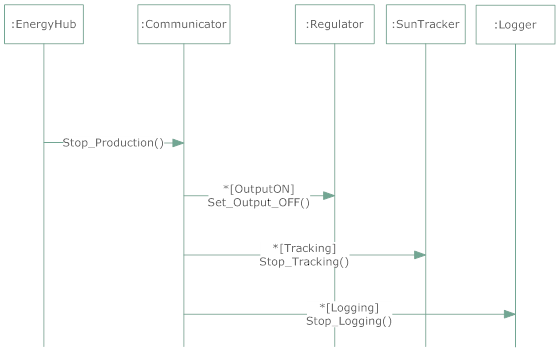
\includegraphics[width=8cm]{images/SequenceDiagram}
\caption{}
\label{fig:SequenceDiagram}
\end{figure}



\subsection{Technical Platform (All)}
The requirements to this project states that we have to use the LPC2478 development board. This board is a piece of hardware, with an ARM7 processor, where the software is written, which has to control the entire system. Besides of that, the hardware interface between the different parts of the system has to be made.


\begin{tabular}{|l|c|c|c|c|}
\hline \textbf{Block} & \textbf{Interface} & \textbf{HW} & \textbf{SW} & \textbf{Mechanics} \\ 
\hline SolarPanel & Analog & X &  &  \\ 
\hline SunTracker & Digital &  & X &  \\ 
\hline Regulator & Ana/dig & X &  &  \\ 
\hline MotorDriver & Ana/Dig & X & X & X \\ 
\hline Communicator & Digital & X &  &  \\ 
\hline Logger & Ana/dig & X & X &  \\ 
\hline PLC & Ana/dig & X & X &  \\ 
\hline 
\end{tabular}


The SolarPanel receives energy from the sun and converts it to electrical energy. This happens inside the hardware of the panel, by the use of semi-conductors. It produces energy and sends it to the regulator.\\

The Regulator regulates the input it receives from the solar panels into the desired voltage/current the energy hub wants to receive from our part of the system. There is no need of software to control the system; this will work by pure hardware.\\

To get the best output from the SolarPanel, it has to point in the right direction. The PositionTracker will find out in which direction the sun is, so it can measure in which directions the panel has to point. This block both requires software and hardware to work properly.\\

The MotorDriver will turn the panel in the right direction, when it receives the position from the SunTracker. The software of this block will compare the panel position with the measured sun position. If they’re not the same, it will turn on the motors, and set the right angle.\\

The Communicator is the communication line to the energy hub. The hub sends signals to start/stop production, and also receive a ping in a given interval, which will test if the connection is on or lost. If it does not receive a ping during the period, it will turn off the system, to ensure not making bad worse. If it doesn’t receive a ping, the communication to the hub is lost and it does not know if it has to stop production or not.\\


\subsection{Contracting}

\subsubsection{Time Schedule (Jacob)}

INSERT SCHEDULE

\subsubsection{Product Acceptance}
The product acceptance is the phase where the requirements are validated. The common requirements and the validation method are to find at:\\
http://e10.ede.hih.au.dk/index.php/Common\_Requirements
\\

\section{Realization Phase}
In the realization phase an analysis of the design, implement it, verify it, and then deploy it. When that have been the realization phase will start over until the product is according to the user needs.  When the realization phase is over and the product is successfully created then we will move on to the Post-Project Phase.\\

\subsection{Strategy and Planning}
\subsubsection{Risk Management}
\textbf{Risk Events (ALL):}\\

When the system-to-be is done, errors can occur. Those errors have to be identified, if possible, and then they can be avoided. Risk events are all the events that can cause the system to either not work properly or even not being realizable.\\


\textit{All system errors}\\

Below are the events that might occur when creating and using our system.

\begin{enumerate}
\item Defect items (Squeak / Rattle) indicated by how many percent of people would notice it, 25\%, 50\% or 75\%.
\subitem The users overall feeling about using the system. Does it sound different from day to day, or are there any parts that may begin to make noise after some time. If such noise appears, how many will notice it, and wonder why it sounds like that?
\item Project can’t be finalized due to budget, time, mechanics or software etc. 
\subitem Maybe the planned budget won’t be big enough, and it is impossible to lend more money, then the project can’t be finalized. Also if time runs out and the deadline can’t be moved the project won’t finish. Also if the mechanics or the software can’t solve the desired problem, all will be lost. Things like these can happen, and sometimes they can’t be solved. Then the project has to be trashed. 
\item Budget overrun
\subitem If there is need for more money, and they can be lent, the project can move on, but with a new budget. This should be avoided, because if the project uses more money than planned, the company loses money they didn’t thought they would lose. 
\item Project time schedule delay
\subitem Of course the customer wants his product in time, so a schedule delay must not occur. If it does, the project crew must talk with the customer and plan a new time. 
\item Customer disappointed with the product
\subitem The customer buys a new product to satisfy his needs, and if the product doesn’t fit to what he expected, he will be disappointed. This can be avoided by communicating and show the progress to the . The mistakes shall be identified as early in the project phase as possible. 
\item Delay in software modifications
\subitem ??
\item Unsupportable software
\subitem ??
\item Solar Panel effectiveness drop more than 10\% in 8 years.
\subitem All solar panels losses effectiveness over years. An average solar panel will have 90\% effectiveness after 10 years of use . The effectiveness of the panel in the system will not drop more than 10\% in the first 8 years. 
\item Dead magnetic spot in engine
\subitem It is possible that the motor stops in a pot, where it can’t start from again. This is called a dead magnetic spot. 
\item Board failure
\subitem During the development process or after the product is finished, the board can break down, due to mistakes from users/developers or failure of the hardware. 
\item Current/voltage readout failure
\subitem When the logger logs the output from the system, a failure can occur, so it skips a measurement. The graph on the web-page will be somewhat more imprecise. 
\item System consumes too much power
\subitem This system is made to save energy for the user, if the system consumes too much energy when collecting solar power, the system would be without purpose. 
\item System burn down due to high voltage
\subitem A high voltage sent the system, occurred from the solar panel or the hub, will damage the system. 
\item Impossible to implement SunTracker
\subitem It is possible that we don’t have the necessary resources to implement the sun tracker to our system. This could be due to time, money or knowledge. 
\item Physical damage
\subitem The panel and the system is placed outside, where physical damage can occur. This could be rocks or fireworks that could damage the panel. 
\item SolarPanel Burn down
\subitem There is a risk that the solar panel could burn-down, just by normal use. 
\item Engine overload
\subitem Obstacles could prevent the solar panel from turning into the right position, this can burn the motors. Those obstacles could be rust or trash. 
\item Inexact motor position
\subitem The motors have to be precise to make the panel point in the right direction. Also the system has to control the motors precisely to get the optimal position. 
\item Software failure
\subitem A failure in the software can reduce the effectiveness of the system, or even damage it badly. 
\item Panel covered by leaves/trash/snow
\subitem The panel shall be placed outside, where leaves and other trash can cover the panel. 
\item SunTracker very inexact
\subitem The sun tracker has to be precise, like the motors, to make the angle to the sun right. If the sun tracker is very inexact, the wrong angle will be measured, and the system will be very ineffective. 
\item Communication failure (SW)
\subitem The communication with the energy hub is very important, this is the line where the safety instructions will be send/received, and the system shall receive those instructions due to safety reasons. 
\item Inexact voltage/current readout
\subitem If the readout of the current/voltage is inexact, the system may transfer too low power to the energy hub, which will cause serious damage. 
\item Components worn-down
\subitem All components will wore-down after some time, but those components which are hard to change, should last for longer than the cheap components that are easy to change. 
\item Emergency button Malfunction
\subitem The emergency button has to function, if it don’t, the safety will be very bad. 
\end{enumerate}


\textbf{Risk Probabilities:}\\

Some events are more likely to occur than other. The events have to be analyzed and given some probability of how likely they will occur.\\

In the table below are the events listed that might occur when using our product compared with the estimated probability that it happens.\\


\begin{landscape}

\begin{tabular}{|l|p{12cm}|p{4cm}|}
\hline Rank & Probability & Estimated Probability (in \%) \\ 

\hline 1 & Unsupportable software \newline 
Project can’t be finalized \newline 
Budget overrun Dead magnetic spot in engine  & Less than 2 \\ 

\hline 2 & Costumer Dissapointed\newline
Major project time schedule delay\newline
SolarPanel Burn-Down\newline
Solar Panel effectiveness drop more than 10\% in 8 years.\newline
Physical Damage (Stone, fireworks etc..)\newline
Impossible to implement SunTracker\newline
System burn down due to high voltage.\newline
System consumes too much power\newline
Current/voltage readout failure\newline
Board failure\newline
Emergency button Malfunction & 2 - 10 \\ 

\hline 3 & Defect (Squeak / Rattle 75\%)\newline
Delay in software modifications\newline
Panel covered by leaves/trash\newline
Software Failure\newline
Inexact motor position\newline
Engine overload & 10 - 20 \\

\hline 4 & Defect (Squeak / Rattle 50\%)\newline
Communication failure (SW)\newline
SunTracker very inexact & 20 – 35 \\

\hline 5 & Inexact voltage/current readout & 35 – 50 \\ 

\hline 6 & Minor project time schedule delay & 50 – 65 \\ 

\hline 7 & Defect (Squeak / Rattle 25\%) & 65 – 75 \\ 

\hline 8 & Components worn-down & 75 – 85 \\ 

\hline 9 &  & 85 – 95 \\ 

\hline 10 &  & 95 – 99.9 \\

\hline 

\end{tabular} 
\end{landscape}

\textbf{Risk impact:}\\

If one of these events occurs in the system, they will have an effect on the functionality of the system. This effect can be minor or major, or somewhere in between. It is a very good idea to analyse the events and find out, how bad it will be if one of the events occurs.\\
In the table below is each event set up with the effect of it occurring.

\noindent \begin{tabular}{|l|p{4cm}|p{10cm}|}
\hline Rank  & Effect & Estimated impact \\ 

\hline 1 \& 2 & None or very minor & Defect items (Squeak / Rattle noticeable by 25\%) \\ 

\hline 3 & Minor & Defect items (Squeak / Rattle noticeable by 50\%)\newline
Schedule delay \textgreater 10\% late\newline
Solar Panel effectiveness drop more than 10\% in 8 years.\newline
 \\ 

\hline 4 & Very low & Defect items (Squeak / Rattle noticeable by 75\%)\newline
Schedule delay \textgreater 10\% late \\ 

\hline 5 & low & Minor delay in software modifications\newline
Customer somewhat disappointed\newline
SunTracker very inexact \\ 

\hline 6 & Moderate & Serious Schedule delay \textgreater 30\% late\newline
Serious budget overrun\newline
Dead magnetic spot in engine\newline
Impossible to implement SunTracker\newline
Inexact motor position\newline
Panel covered by leaves/trash\newline
Slightly Inexact voltage/current readout\newline
Components worn-down \\ 

\hline 7 & High & Customer very disappointed\newline
Board failure \\ 

\hline 8 & Very High & Major delay In software modifications \newline
Large schedule delay \textgreater 40\% late\newline
Current/voltage readout failure\newline
System consumes too much power\newline
Physical damage\newline
SolarPanel Burn down\newline
Engine overload\newline
Software failure\newline
Communication failure (SW)\newline
Very Inexact voltage/current readout \\ 

\hline 9 & Hazardous with warning & Major budget overrun\newline
Unsupportable software\newline
Project can’t be finalized \\ 

\hline 10 & Hazardous without warning & System burn down due to high voltage\newline
Emergency button Malfunction \\ 

\hline 
\end{tabular} 
\\

\textbf{Possibility of detection before release:}\\

A analyze of how possible it is to detect a problem before the release of the product also has to be made. As an example, it is sometimes hard to detect how stable the software is, before the system has been on for some time. But if it a minor delay in the software, it is much more likely to be discovered before release.\\
In the table below each event is paired with the estimated chance to detect it in percent.\\

\noindent\begin{tabular}{|l|p{10cm}|p{4cm}|}
\hline Rank & Probability & Estimated Probability\newline (in \%) \\ 

\hline 10 &  & Less than 2 \\ 

\hline 9 &  & 2 - 10 \\ 

\hline 8 & Components worn-down & 10 -20  \\ 

\hline 7 & Defect items (Squeak / Rattle noticeable by 25\%) & 20 - 35 \\ 

\hline 6 &Project time schedule delay  \textgreater 10\% \newline
Project time schedule delay \textgreater 10\%  & 35 - 50 \\ 

\hline 5 & Slightly Inexact voltage/current readout\newline
Very Inexact voltage/current readout & 50 - 65 \\ 

\hline 4 & Defect items (Squeak / Rattle noticeable by 50\%)\newline
SunTracker very inexact & 65 - 75 \\ 

\hline 3 & Defect items (Squeak / Rattle noticeable by 75\%)\newline
Minor delay in software modifications\newline
Major delay in software modifications\newline
Engine overload\newline
Inexact motor position\newline
Software failure\newline
Panel covered by leaves/trash\newline
Communication failure (SW) & 75 - 85 \\ 

\hline 2 & Project time schedule delay \textgreater 30\%\newline
Project time schedule delay \textgreater 40\%\newline
Customer disappointed\newline
Solar Panel effectiveness drop more than 10\% in 8 years.\newline
Board failure\newline
Current/voltage readout failure\newline
Emergency button Malfunction\newline
System consumes too much power\newline
System burn down due to high voltage\newline
Impossible to implement SunTracker\newline
Physical damage\newline
SolarPanel Burn down & 85 - 95  \\ 

\hline 1 & Project can’t be finalized\newline
Serious budget overrun\newline
Large budget overrun\newline
Unsupportable software\newline
Dead magnetic spot in engine & 95 - 99.9 \\ 

\hline 
\end{tabular} 


\textbf{Risk Rank}\\

In the table below the risk rank is calculated from the formula:
\\
Probability rank * Impact rank * detection rank the higher the rank risk - the greater problem is said event for us. Range is from 1 – 1000.\\
\noindent
\begin{tabular}{|p{10cm}|p{1cm}|p{1cm}|p{1cm}|p{1cm}|}
\hline Event  & \begin{sideways}Probability Rank\end{sideways} & \begin{sideways}Impact Rank\end{sideways} & \begin{sideways}Detection Rank\end{sideways} & \begin{sideways}Risk Rank (*)\end{sideways} \\ 
\hline Defect items (Squeak / Rattle noticeable by 25\%) & 7 & 1 & 7 & 49 \\ 
\hline Defect items (Squeak / Rattle noticeable by 50\%) & 4 & 3 & 5 & 60 \\ 
\hline Defect items (Squeak / Rattle noticeable by 75\%) & 3 & 4 & 3 & 36 \\ 
\hline Project can’t be finalized & 1 & 10 & 1 & 10 \\ 
\hline Serious budget overrun & 1 & 6 & 1 & 6 \\ 
\hline Large budget overrun & 1 & 10 & 1 & 10 \\ 
\hline Project time schedule delay \textless 10\% & 6 & 3 & 1 & 18 \\ 
\hline Project time schedule delay \textgreater 10\% & 6 & 4 & 1 & 24 \\ 
\hline Project time schedule delay \textgreater 30\% & 2 & 6 & 1 & 12 \\ 
\hline Project time schedule delay \textgreater 40\% & 2 & 8 & 1 & 16 \\ 
\hline Customer disappointed & 2 & 5 & 9 & 70 \\ 
\hline Minor delay in software modifications & 3 & 5 & 8 & 120 \\ 
\hline Major delay in software modifications & 3 & 8 & 2 & 48 \\ 
\hline Unsupportable software & 1 & 10 & 1 & 10 \\ 
\hline Solar Panel effectiveness drop more than 10\% in 8 years & 2 & 3 & 10 & 60 \\
\hline Dead magnetic spot in engine & 1 & 6 & 10 & 60 \\ 
\hline Board failure & 2 & 7 & 9 & 126 \\ 
\hline \textcolor{green} {Current/voltage readout failure} & 2 & 8 & 10 & 160 \\ 
\hline System consumes too much power & 2 &  2 & 8 & 32 \\ 
\hline \textcolor{red} {System burn down due to high voltage} & 2 & 10 & 10 & 200 \\ 
\hline Impossible to implement SunTracker & 2 & 6 & 1 & 12 \\ 
\hline \textcolor{green} {Physical damage} & 2 & 8 & 10 & 160 \\ 
\hline \textcolor{green} {SolarPanel Burn down} & 2 & 8 & 10 & 160 \\ 
\hline \textcolor{red} {Engine overload} & 3 & 8 & 9 & 216 \\ 
\hline Inexact motor position & 3 & 6 & 10 & 180 \\
\hline Software failure & 3 & 8 & 2 & 48 \\ 
\hline \textcolor{yellow}{Panel covered by leaves/trash} & 3 & 6 & 10 & 180 \\ 
\hline SunTracker very inexact & 4 & 5 & 1 & 20 \\ 
\hline Communication failure (SW) & 4 & 8 & 4 & 128 \\ 
\hline Slightly Inexact voltage/current readout & 5 & 6 & 4 & 120 \\ 
\hline \textcolor{green} {Very Inexact voltage/current readout} & 5 & 8 & 4 & 160 \\ 
\hline \textcolor{red} {Components worn-down} & 8 & 6 & 9 & 432 \\ 
\hline Emergency button Malfunction & 2 & 10 & 7 & 140 \\ 
\hline 
\end{tabular} 

*[Risk Rank] = [Probability Rank]<[Impact Rank]x[Detection Rank]
\\
\textcolor{green} {Important}
\\
\textcolor{yellow} {More important}
\\
\textcolor{red} {Most important}
\\

\textbf{Risk Rank Diagram:}\\

In the diagram below a color code system is used, where green is risks with low probability and low impact, yellow is either low probability high impact or high probability low impact, while red is high impact and impact probability. X axis is increasing probability and Y axis is increasing Impact.  The numbers indicate how much impact rank or probability rank the event has.\\


\begin{tabular}{|p{1cm}|p{5.5cm}|p{5.5cm}|p{5.5cm}|}
\hline 8-10 & Unsupportable Software\newline
Major Delay in software modifications \newline
Project schedule time delay \textgreater 30\% \newline
Large budget overrun \newline
Project can’t be finalized \newline
Current/voltage readout failure \newline
System consumes too much power \newline
System burn down due to high voltage \newline
Impossible to implement SunTracker \newline
Physical damage \newline
SolarPanel burn down \newline
Engine overload \newline
Inexact motor position \newline
Software failure \newline
Communication failure (SW) \newline
Emergency button Malfunction & Reduced performance \newline
Very Inexact voltage/current readout &  \\

\hline 5-7 & Minor delay In software modifications\newline
Customer disappointed\newline
Defect items (Squeak / Rattle 50\%)\newline
Dead magnetic spot in engine\newline
Board failure\newline
Panel covered by leaves/trash & Slightly Inexact voltage/current readout & Components worn-down \\ 

\hline 0-4 & Solar Panel effectiveness drop more than 10\% in 8 years. & Project time schedule delay \textgreater 10\% \newline
Defect items (Squeak / Rattle 75\%) & Defect items (Squeak / Rattle 25\%) \\ 

\hline  & 0-4 & 5-7 & 8-10 \\ 

\hline 
\end{tabular} 


A quick analyse of this diagram shows that we have a lot of events with a high impact on our system but luckily a low probability rank of it happening, while the things with most probability of happening are Defect items (Squeak / Rattle) where around 25\% notice it and are annoyed by it and Components worn-down. The best thing that can be seen from this diagram is that there are no events with a high probability and a high impact that could occur for our system.\\


\textbf{Development Strategy (Henrik)}\\

The central part in the system to be is the microprocessor, which in this case is the LPC-2478 board. This is because it controls most of the other parts of the system; therefore it is a good choice for a starting point, as it allows for other parts of the system to be developed earlier in the process.\\

The SunTracker will be one of the more time consuming parts. Therefore it must be started early in the process to make sure it will be developed in time according to schedule.\\

Some of the biggest risk impacts in the system are:
\begin{itemize}
\item Components worn down
\item Engine overload
\item System burn-down due to high voltage/current/something
\item Panel covered by leaves/trash
\item Physical damage to panel
\item Current/voltage readout failure
\item Solar panel burn-down
\item Very inexact voltage/current readout
\end{itemize}

These are risks that need to be included in early stages of the development process to take necessary precautions and minimize the probability that they will occur. The risks can be cooked down to the following topics:\\


\begin{itemize}
\item Choice of components
\item Current check on motors
\item Emergency systems
\item Shielding (position and protection) hardware
\end{itemize}


Solar panel burn-down/malfunction can only be avoided by using the best possible solar panels. This project is aimed for an already existing solar panel, so there can be taken no precautions about this.\\

The power line communication sets certain requirements to the system. This, however, is a task to be solved in cooperation with the other teams; therefore it will only have medium-high priority in the time planning.
Errors found are put on an error list and qualified, later to be corrected.\\

Error list
\begin{tabular}{|l|l|l|}
\hline Timebox(week) & Error & Category \\ 
\hline 48-49 &  &  \\ 
\hline 
\end{tabular} 	

New ideas shall be noted, later to be discussed whether to implement or not.\\

Idea list

\begin{tabular}{|l|l|l|}
\hline Timebox(week) & Error & Category \\ 
\hline 48-49 &  &  \\ 
\hline 
\end{tabular} 

\end{document}